% =============================================================================

\vspace*{\fill}

\begin{figure}[!h]
\begin{lstlisting}[language=pseudo,style=block]
saes.v4.ks1       rd rs1 rcon : v4.ks1(rd, rs1, rcon)
saes.v4.ks2       rd rs1 rs2  : v4.ks2(rd, rs1, rs2 )
saes.v4.imix      rd rs1      : v4.InvMix(rd, rs1)
saes.v4.encsm     rd rs1 rs2  : v4.Enc(rd, rs1, rs2, mix=1)
saes.v4.encs      rd rs1 rs2  : v4.Enc(rd, rs1, rs2, mix=0)
saes.v4.decsm     rd rs1 rs2  : v4.Dec(rd, rs1, rs2, mix=1)
saes.v4.decs      rd rs1 rs2  : v4.Dec(rd, rs1, rs2, mix=0)
\end{lstlisting}
\caption{
  Instruction mnemonics, and their mapping onto pseudo-code functions, for \ISE{4}.
}
\label{fig:v4:mnemonics}
\end{figure}

\begin{figure}[!h]
\begin{lstlisting}[language=pseudo,style=block]
v4.ks1(rd, rs1, enc_rcon):     // KeySchedule: SubBytes, Rotate, Round Const
    temp.32   = rs1.32[1]
    rcon      = 0x0
    if(enc_rcon != 0xA):
        temp.32 = ROTR32(temp.32, 8)
        rcon    = RoundConstants.8[enc_rcon]
    temp.8[i] = AESSBox[temp.8[i]]  for i=0..3
    temp.8[0] = temp.8[0] ^ rcon
    rd.64     = {temp.32, temp.32}

v4.ks2(rd, rs1, rs2):           // KeySchedule: XOR
    rd.32[0]  = rs1.32[1] ^ rs2.32[0]
    rd.32[1]  = rs1.32[1] ^ rs2.32[0] ^ rs2.32[1]

v4.Enc(rd, rs1, rs2, mix): // SubBytes, ShiftRows, MixColumns
    t1.128    = ShiftRows({rs2, rs1})
    t2.64     = t1.64[0]
    t3.8[i]   = AESSBox[t2.8[i]] for i=0..7
    rd.32[i]  = AESMixColumn(t3.32[i]) if mix else t3.32[i] for i=0..1

v4.Dec(rd, rs1, rs2, mix, hi): // InvSubBytes, InvShiftRows, InvMixColumns
    t1.128    = InvShiftRows(rs2 || rs1)
    t2.64     = t1.64[0]
    t3.8[i]   = AESInvSBox[t2.8[i]] for i=0..7
    rd.32[i]  = AESInvMixColumn(t3.32[i]) if mix else t3.32[i] for i=0..1

v4.InvMix(rd, rs1):             // Inverse MixColumns
    rd.32[i]  = AESInvMixColumn(rs1.32[i]) for i=0..1
\end{lstlisting}
\caption{
  Instruction pseudo-code functions for \ISE{4}.
}
\label{fig:v4:pseudo}
\end{figure}

\begin{figure}[!h]
\begin{lstlisting}[language=pseudo,style=block]
ld              a0, 0(a4)  // Load round key as double words.
ld              a1, 8(a4)
xor             t0, t0, a0 // Add round key for 2 columns at a time.
xor             t1, t1, a1
aes.v5.encsm    t2, t0, t1 // Next round state: columns 0, 1
aes.v5.encsm    t3, t1, t0 // columns 2, 3 - Note swapped rs1/rs2
\end{lstlisting}
\caption{
  An AES encryption round implemented using \ISE{4}.
}
\label{fig:v4:round}
\end{figure}

\vspace*{\fill}

% -----------------------------------------------------------------------------

\newpage

\vspace*{\fill}

\begin{figure}[!h]
\centering
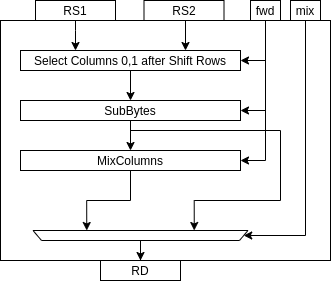
\includegraphics[width={0.5\textwidth}]{diagrams/ise-datapath-v4.png}
\caption{
  A diagramatic description of the functional unit required to support the
  \ISE{4} round instructions.
}
\label{fig:v4:fu}
\end{figure}

\vspace*{\fill}

% =============================================================================
